From the experimental results in subsection \ref{subsec: Result and Analysis}, we can see that when there is enough information, the Level Set method can achieve a precise segmentation result. However, when the scene of the picture is more complex, the Level Set method cannot achieve the desired segmentation result, and some \textbf{pattern recognition} methods are needed to bring more information about the target, for example, where is the target regions, and the probability that each pixel belongs to the target category. In the process of contour evolution, it relies on the statistic of pixels inside and outside the contour with fixed $\phi$ at this time, such as mean \cite{LevelSet:chan2001active}, weighted mean \cite{LevelSet:mathod:li2008minimization}, and probability model about regions \cite{LevelSet:Discussion:lin2005probability}. The Level set method is more like an integration of information, using energy functional minimization principle to construct a potential function based on those information. And this potential function can have a higher meaning, such as probability, so that we can add probabilities and Bayesian methods.

In this paper, the GAT is used to find the optimal affine transformation of the standard prior shape based on the probability map. But it is based on the contour, and the probability map expresses the regions, so when the result of FCNs are poor, the GAT will fail to match. The failure result of the GAT is shown in Fig. \ref{fig: The failure result of the GAT}.
\begin{figure}[h]
    \centering
    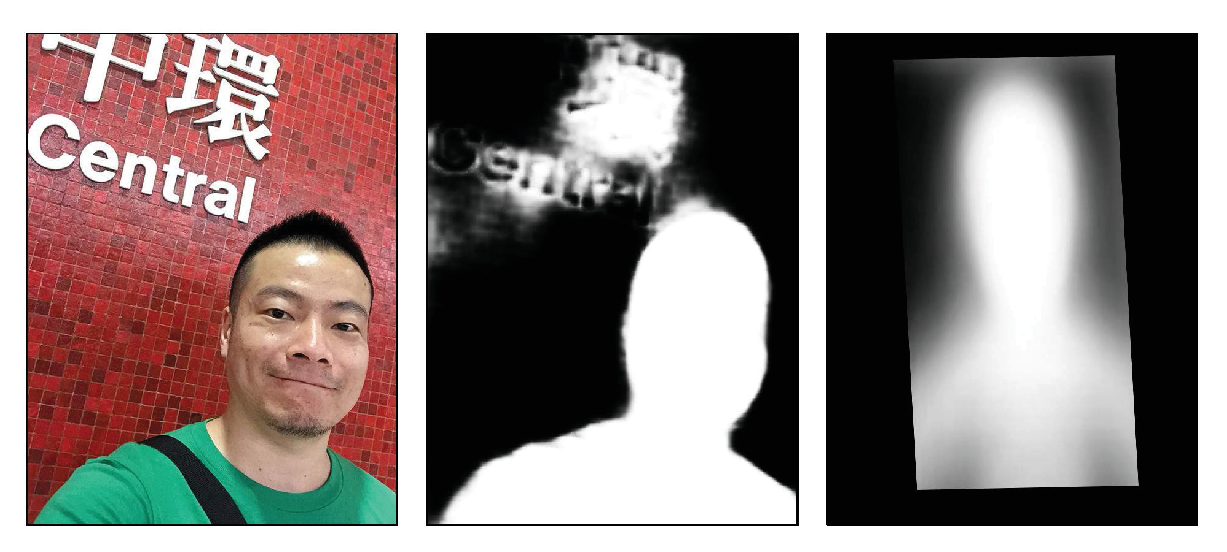
\includegraphics[width=7cm]{figs/GAT_Failed.eps}
    \caption{The failure result of the GAT.}
    \label{fig: The failure result of the GAT}
\end{figure}

Even if the pixels are very similar, the imprecise probability map and corrected prior shape still have a large effect, causing similar pixels are split apart. But we can draw on the idea of superpixels \cite{LevelSet:superpixels:achanta2012slic}. Most of the methods can be summarized as how to extract and use the information in images, so the most important issue is to build the dynamic hierarchial structured representation of images. 